%%%%%%%%%%%%%%%%%%%%%%%%%%%%%%%%%%%%%%%%%%%%%%%%%%%%%%%%%%%%%%%%%%%%%%
%
% Institut für Rechnergestuetzte Automation
% Forschungsgruppe Industrial Software
% Arbeitsgruppe ESSE
% http://security.inso.tuwien.ac.at/
% lva.security@inso.tuwien.ac.at
%
% Version 2014-04-10
% 
%%%%%%%%%%%%%%%%%%%%%%%%%%%%%%%%%%%%%%%%%%%%%%%%%%%%%%%%%%%%%%%%%%%%%%

\documentclass[12pt,a4paper,titlepage,oneside]{scrartcl}
\usepackage{esseProtocol}

%%%%%%%%%%%%%%%%%%%%%%%%%%%%%%%%%%%%%%%%%%%%%%%%%%%%%%%%%%%%%%%%%%%%%%
%
% FOR STUDENTS
%
%%%%%%%%%%%%%%%%%%%%%%%%%%%%%%%%%%%%%%%%%%%%%%%%%%%%%%%%%%%%%%%%%%%%%%

% Group number or "0" for Lab0
\newcommand{\gruppe}{2}
% Date
\newcommand{\datum}{2014-05-16}
% valid values: "Lab0", "Lab1" (be sure to use Uppercase for first character)
\newcommand{\lab}{Lab1}

% name of course
\newcommand{\lvaname}{IT Security in Large IT Infrastructures}
% number of course
\newcommand{\lvanr}{183.633}
% year and term, for example: "SS 2012", "WS 2012", "SS 2013", etc.
\newcommand{\semester}{SS 2014}

% Student data in Lab0 or 1. student of group in Lab1
\newcommand{\studentAName}{Ren\'{e} Czerny}
\renewcommand{\studentAMatrnr}{0825750}
\newcommand{\studentAEmail}{e0825750@student.tuwien.ac.at}

% 2. student of group in Lab1, for Lab0 or if your group has less students, remove these 3 lines
\newcommand{\studentBName}{Andreas Riegler}
\renewcommand{\studentBMatrnr}{1028878}
\newcommand{\studentBEmail}{e1028878@student.tuwien.ac.at}

% 3. student of group in Lab1, for Lab0 or if your group has less students, remove these 3 lines
\newcommand{\studentCName}{Klaus Walla}
\renewcommand{\studentCMatrnr}{1028877}
\newcommand{\studentCEmail}{e1028877@student.tuwien.ac.at}

%%%%%%%%%%%%%%%%%%%%%%%%%%%%%%%%%%%%%%%%%%%%%%%%%%%%%%%%%%%%%%%%%%%%%%
%
% DO NOT CHANGE THE FOLLOWING PART
%
%%%%%%%%%%%%%%%%%%%%%%%%%%%%%%%%%%%%%%%%%%%%%%%%%%%%%%%%%%%%%%%%%%%%%%

\newcommand{\lang}{de}
\newcommand{\colormode}{color}
\newcommand{\dokumenttyp}{Abgabedokument \lab}

\begin{document}

\maketitle
\setcounter{section}{0}
\setcounter{tocdepth}{2}
\tableofcontents

%%%%%%%%%%%%%%%%%%%%%%%%%%%%%%%%%%%%%%%%%%%%%%%%%%%%%%%%%%%%%%%%%%%%%%
%
% CONTENT OF DOCUMENT STARTS HERE
%
%%%%%%%%%%%%%%%%%%%%%%%%%%%%%%%%%%%%%%%%%%%%%%%%%%%%%%%%%%%%%%%%%%%%%%

\section{Lab1a}

\subsection{Report}
\textbf{Speicherung des Passworts mangelhaft (OWASP A7):}
In der Anwendung wird ein SHA1-Hash f\"ur die Speicherung des Passworts in die Datenbank verwendet, wodurch zu allen gespeicherten Hashes mittels beispielsweise Rainbow-Tabellen in ausreichend lohnenswerter Zeit der passende Klartext gefunden werden kann. Weit aus sicherer wäre es, wenn ein stärkeres Hashverfahren z.B. SHA256 in Kombination eines Salts verwendet werden würde.
\newline
\newline
\textbf{Sicherheitsrelevante Fehlkonfiguration (OWASP A6):}
Directory Listing ist in der Anwendung nicht deaktiviert. Angreifer können einfach im Verzeichnis des Servers navigieren und so alle Pythonklassen und die Datenbank herunterladen und somit verschiedenste Schwachstellen durch Code- bzw. Datenbankanalyse herausfiltern. Im speziellen können alle unverschlüsselt gespeicherten Daten(Usernamen, Events,…) aus der Datenbank gelesen werden, da die SqlLite-Datenbank nicht mittels Passwort verschlüsselt werden kann. 
\newline
\newline
\textbf{Unzureichende Absicherung der Transportschicht (OWASP A9):}
Die Authentifizierung erfolgt ohne TLS/SSL, wodurch die Anmeldeinformationen im Netzwerkverkehr für jeden im Klartext ersichtlich wären. Angreifer könnten diesen einfach sniffen und so Zugang zu dem Benutzerkonto erhalten. Auch für die Textkommunikation wäre die Verwendung von TLS/SSL sinnvoll bzw. erforderlich, da es sich um sensible Daten handelt.
\newline
\newline
\textbf{Fehler im Sessionmanagement (OWASP A3):}
Im Zuge des Sessionmanagements wurden gleich einige Fehler gemacht. Erstens wurden die Session-IDs in der URL mitgeschickt und zweitens wurden diese auch ungeschützt (ohne TLS/SSL) übertragen, wodurch Angreifer einfach die Session des Benutzers übernehmen können(Session Hijacking), wenn Angreifer Zugriff auf den relevanten Netzverkehr haben und diesen ausliest. Durch die Speicherung der Session in der URL ist es schon gefährlich, wenn der Benutzer unvorsichtig diese als Link an Freunden schickt, welche dann (möglicherweise unbewusst) seine Session übernehmen. Verhindert werden kann das, indem die Session-ID erstens nicht in der URL übertragen wird, sondern nur über TLS/SSL gesicherte Transportwege bzw. über ein Cookie mit gesetztem Secure-Flag. 
Des weiteren wurde die Zeit  für das Auslaufen der Session viel zu lang spezifiziert (6000s=1h 40min). Nachfolgende Benutzer des Browsers können bei unzureichendem Logout(einfaches Schließen des Browsers) einfach weiterhin die Session des zuvor angemeldeten Users verwenden. Zusätzlich besteht bei der ursprünglichen Chatterboxanwendung nicht einmal die Möglichkeit eine Abmeldung des Users durchzuführen.
\newline
\newline
Verfügbarkeit: Neben den Sicherheitslücken wurde auch ein ausnutzbarer Programmierfehler für einen Denial of Service DOS-Attacke entdeckt. Wird nämlich kein Alias angeben stürzt der Server ab, wodurch für jegliche User dieser unerreichbar wird.

\subsection{Example exploit}
ChatterBox in der jetztigen Version ist anf"allig f"ur Session Hijacking. Da die gesamte Daten"ubertragung unverschl"usselt erfolgt kann ein Angreifer z.B. mittels Packet Sniffing Session-IDs stehlen oder auch sogar an Login-Daten gelangen.
\newline
\newline
Beispiel:
\newline
Ein Benutzer loggt sich "uber ein unverschl"usseltes WLAN an einem ChatterBox-Server ein. Ein Angreifer k"onnte nun den Datenverkehr mithilfe eines Packet Sniffers (z.B. Wireshark) mitlesen und so die Session-ID, die bei jedem HTTP-Request/Response mitgeschickt wird, dieses Benutzers erhalten (\hyperref[fig:message]{siehe Abbildung~\ref*{fig:message} auf Seite~\pageref*{fig:message}}).
\begin{figure}[h!]
  \centering
  \fbox{
    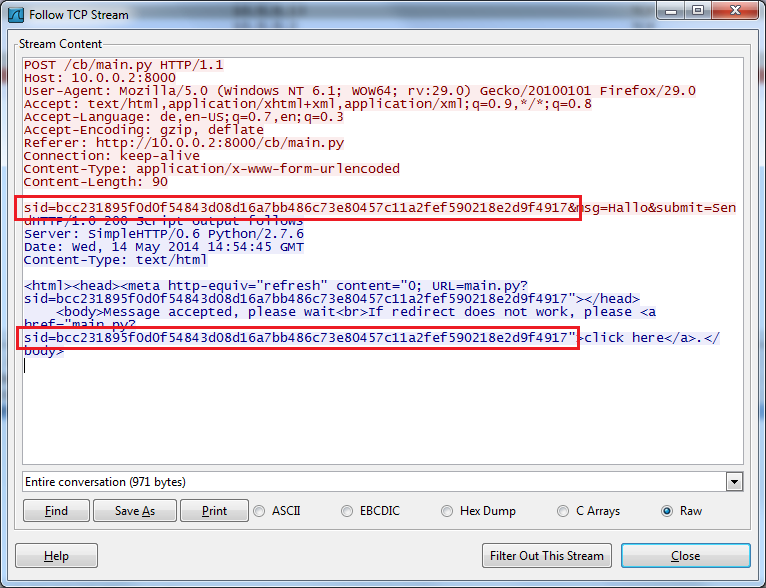
\includegraphics[width=0.8\textwidth]{./imgs/send_message.png}
  }
  \caption{Benutzer schickt eine Message ab}
  \label{fig:message}
\end{figure}
\newline
\newline
Mittels dieser Session-ID erh"alt der Angreifer nun Zugriff auf den Account des Benutzers indem er die gestohlene ID "uber die URL angibt (\lstinline{http://<Server-IP>:8000/cb/main.py?sid=<gestohlene SID des Benutzers>}).

\subsection{Executive summary}
Die Chatterbox Applikation wurde einer gr"undlichen Security-Untersuchung unterzogen, bei der schwere Sicherheitsm"angel festgestellt wurden. In der jetzigen Form sind Vertraulichkeit, Integrit"at und Verf"ugbarkeit der Daten gef"ahndet und von einer Verwendung wird dringend abgeraten. Viele dieser M"angel gehen auf Fehler in der Design-Phase von Chatterbox zur"uck, weshalb sich zusammenfassend feststellen l"asst, dass aufgrund teilweise schwerwiegender Sicherheits-Mängel der Chatterbox Applikation - unter anderem fehlender Beachtung von Vertraulichkeit, Integrität und Verfügbarkeit - zu einer grundlegenden Neuprogrammierung geraten wird.

\section{Lab1b}

Um die erkannten Schwachstellen schon in der Design-Phase des Projekts kategorisch auszumerzen, gibt es drei Design-Ziele zu verfolgen, n\"amlich die sogenannte CIA-Triade (Confidentiality, Integrity, Availability - zu deutsch Vertraulichkeit, Integrit\"at, Verf\"ugbarkeit). Mit dem Fokus auf diesen Zielen m\"ochten wir nun eine sichere Basis und Ausgangspunkt f\"ur die Neuentwicklung von Chatterbox erstellen.

\subsection{Confidentiality}
Um confidentiality - Vertraulichkeit zu gew\"ahrleisten ist es essentiell, dass nur der/die gew\"unschte/n Empf\"anger die Nachricht lesen k\"onnen. Es darf nicht m\"oglich sein, dass ein Dritter heimlich oder offensichtlich die Nachricht abfangen und lesen kann. Das beste Mittel zur Vertraulichkeit ist die Verschl\"usselung. Durch das Verschl\"usseln der Nachrichten, kann sie nur von jemandem gelesen werden, der den Schl\"ussel hat und das sind lediglich die Personen, die in einem gemeinsamen Chatroom sind. Ein Dritter w\"urde lediglich die verschl\"usselte Nachricht erhalten, mit der er nichts anfangen kann. Eine Nachricht beinh\"alt auch eine Kennung f\"ur den Absender, die mitverschl\"usselt wird, um sicherzustellen, dass der angebliche Absender auch der tats\"achliche Absender ist. Damit ist die Vertraulichkeit gew\"ahrleistet. (\hyperref[fig:encryption]{siehe Abbildung~\ref*{fig:encryption}})

\subsection{Integrity}
Die Integrit\"at beschreibt die Eigenschaft, dass die Nachricht, die versendet wird auch tats\"achlich jene Nachricht ist, die ankommen wird. Sie darf auf dem Weg weder durch Dritte noch durch irgendwelche Fehler ver\"andert werden. Um dies zu gew\"ahrleisten bedienen wir uns einer Hash-Summe, die f\"ur einen gegebenen Absender und den Text eindeutig ist. Am Ziel wird die Hashsumme erneut berechnet und mit der \"ubertragenen Hash-Summe verglichen. Stimmt der Wert \"uberein, so ist die Integrit\"at gew\"ahrleistet. Damit die Hash-Summe nicht ver\"andert werden kann wird diese in der Nachricht mitverschl\"usselt. (\hyperref[fig:encryption]{siehe Abbildung~\ref*{fig:encryption}})

\begin{figure}[h!]
  \centering
    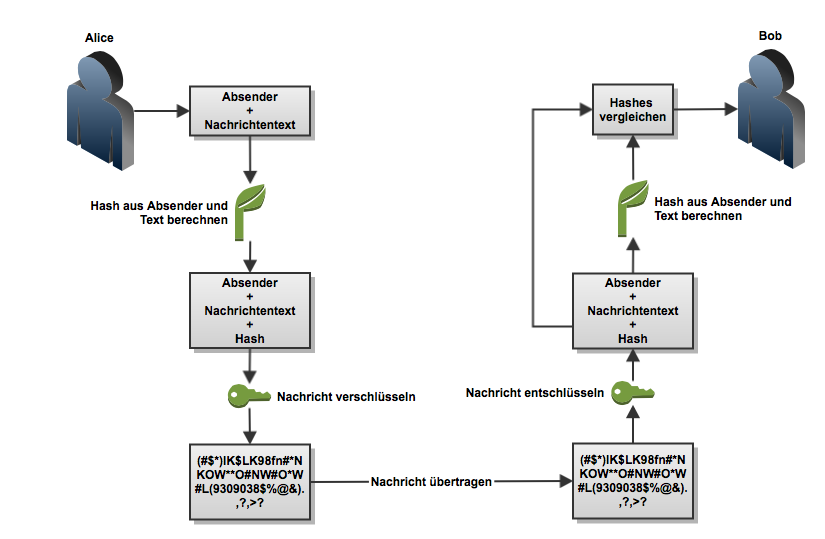
\includegraphics[width=1.0\textwidth]{./imgs/encryption.png}
  \caption{Verschl\"usselung und Hashing}
  \label{fig:encryption}
\end{figure}

\subsection{Availability}
Um Availability - Verf\"ugbarkeit zu gew\"ahrleisten darf das System nicht von einem einzigen Punkt abh\"angen. In der vorigen Version gab es f\"ur Chatterbox nur einen Server. Dies ist f\"ur diesen Anwendungsfall im Kontext der Verf\"ugbarkeit sehr unvorteilhaft. Damit ist der Server ein "Single-Point-Of-Failure" und rei"st bei einem Absturz das ganze System mit sich mit. Um dem vorzubeugen bedienen wir uns der P2P(Peer-To-Peer)-Technologie, in der die Clients direkt miteinander kommunizieren k\"onnen. Damit f\"uhrt der Absturz einer Maschine nicht zum Absturz des gesamten Chat-Netzwerks. (\hyperref[fig:p2p]{siehe Abbildung~\ref*{fig:p2p}})

\begin{figure}[h!]
  \centering
    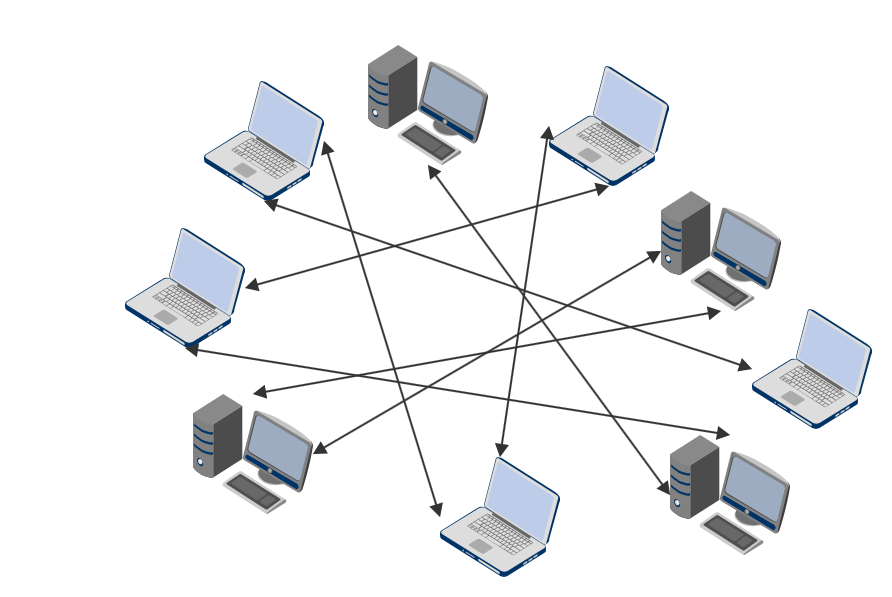
\includegraphics[width=1.0\textwidth]{./imgs/p2p.png}
  \caption{P2P-Netzwerk}
  \label{fig:p2p}
\end{figure}

\newpage
\subsection{Verwendete Technologie}

\subsubsection{Java}
Als Programmiersprache wird Java verwendet. Dies erm\"{o}glicht eine Plattformunabh\"{a}ngigkeit und damit eine einfache Verbreitung der Software auf verschiedensten Plattformen

\subsubsection{JXTA/JXSE}
Zur Umsetzung der P2P-Technologie wird JXTA, bzw. die Java-Implementierung davon JXSE, verwendet. Die JXSE-Pattform erlaubt es uns auf bestehende und erprobte Umsetzungen des Peer-To-Peer Konzepts zur\"{u}ckzugreifen und abstrahiert dadurch einiges an Arbeit und m\"{o}glichen Problemen weg.

\subsubsection{Bouncy Castle Provider}
Als moderner Anbieter diverser Sicherheitstechnologien und -Algorithmen verwenden wir Bouncy Castle zur Umsetzung der Verschl\"{u}sselung und des Hashings.


\subsection{Executive Summary}
Um Chatterbox als sichere Applikation neu zu designen haben wir uns auf die drei wichtigsten Sicherheitsziele konzentriert: Vertraulichkeit, Integrit\"at und Verf\"{u}gbarkeit.
\begin{itemize}
\item \textbf{Vertraulichkeit} - also die Eigenschaft, dass kein Unbefugter die Nachricht lesen kann - wird mittels modernster Verschl\"{u}sselung gew\"{a}hrleistet
\item \textbf{Integrit\"{a}t} - hier wird sichergestellt, dass die Nachricht nicht manipuliert werden kann und original beim Empf\"{a}nger ankommt - wird sichergestellt indem ein Hash-Verfahren verwendet wird, dass den Originalzustand der Nachricht  sicherstellt.
\item \textbf{Verf\"{u}gbarkeit} - die Eigenschaft dass das Chatterbox-System m\"{o}glichst stabil und robust l\"{a}uff und die Ausfallquote minimalst gehalten wird - wird gew\"{a}herleitet, indem der ``Single-Point-Of-Failure'' ausgemerzt wird. So wird sichergestellt, dass das System weiterhin problemlos laufen kann, auch wenn ein oder mehrere Maschinen abst\"{u}rzen.
\end{itemize}
Auf diese Weise kann Chatterbox als sichere Chat-Applikation verwendet werden und der User darauf vertrauen, dass seine Kommunikation die Sicherheit bekommt, die sie verdient.

%%%%%%%%%%%%%%%%%%%%%%%%%%%%%%%%%%%%%%%%%%%%%%%%%%%%%%%%%%%%%%%%%%%%%%
%
% DO NOT CHANGE THE FOLLOWING PART
%
%%%%%%%%%%%%%%%%%%%%%%%%%%%%%%%%%%%%%%%%%%%%%%%%%%%%%%%%%%%%%%%%%%%%%%

\end{document}


